\chapter{Tools}


\section{Serial Terminal} \hypertarget{def:sterm}{}

Open the serial terminal (with system application associated with .sterm file extension ), the default application is the 
\href{https://github.com/neundorf/CuteCom}{Cutecom}. 

\begin{figure}[H]
\center
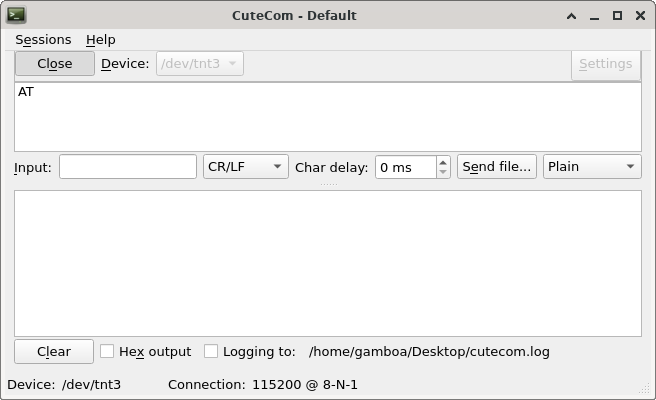
\includegraphics[width=0.8\textwidth]{img/cutecom.png} 
\end{figure} 

A serial terminal is used to send and receive data over a serial communication channel. 
The use of this terminal can be replaced by others like the Arduino IDE serial monitor. 

To use this tool with PICSimLab you first need to configure a virtual serial port as described in Chapter: \hyperlink{def:seriali}{Serial Communication}.
It is possible to use this tool with a real serial port connected to a real device. 


\section {Serial Remote Tank} \hypertarget{def:srtank}{}


The serial remote tank is a tank simulator controlled by a serial communication protocol.
The tank has several sensors and actuators that can be read and controlled using the communication protocol. 
The parameters of the serial communication port must be  19200 8N1. 

\begin{figure}[H]
\center
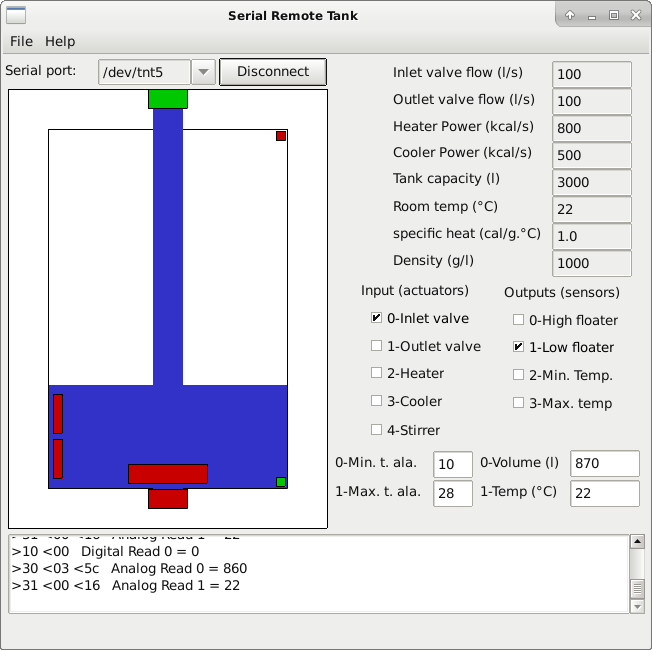
\includegraphics[width=0.8\textwidth]{img/srtank.png} 
\end{figure} 


To use this tool with PICSimLab you first need to configure a virtual serial port as described in Chapter: \hyperlink{def:seriali}{Serial Communication}.
It is possible to use this tool with a real serial port connected to a real device. 

\subsection{Actuators}

Digital inputs:
\begin{enumerate}
\item Inlet valve
\item Outlet valve
\item Heater
\item Cooler
\item Stirrer
\end{enumerate}

Analog inputs:
\begin{enumerate}
\item Minimal temperature alarm trigger level
\item Maximal temperature alarm trigger level
\end{enumerate}

\subsection{Sensors}

Digital outputs:
\begin{enumerate}
\item High floater 
\item Low floater
\item Minimal temperature 
\item Maximal temperature
\end{enumerate}

Analog outputs:
\begin{enumerate}
\item Volume
\item Temperature
\end{enumerate}


\subsection{Communication Protocol}

\subsubsection{Writing on Digital Input}
Sent one byte in 0x0N hexadecimal format where N  is the number of input followed by a second byte with value 0x00 for disable or 0x01 for enable.  

Example to turn on the input 2:
\begin{minted}[baselinestretch=1.2,fontsize=\footnotesize,bgcolor=colorbash]{c}
            Serial_write(0x02);
            Serial_write(0x01);
\end{minted}


\subsubsection{Reading Digital Output}
Sent one byte in 0x1N hexadecimal format where N  is the number of output and read one byte. The byte readed have value 0x00 for disable or 0x01 for enable. 

Example to read output 3:
\begin{minted}[baselinestretch=1.2,fontsize=\footnotesize,bgcolor=colorbash]{c}
      Serial_write(0x13);
      valor=Serial_read(0);
\end{minted}


\subsubsection{Writing on Analog Input} 
Sent one byte in 0x2N hexadecimal format where N  is the number of input followed by two bytes with the 16 bits value.

Example to write the value 230 on analog input 1:
\begin{minted}[baselinestretch=1.2,fontsize=\footnotesize,bgcolor=colorbash]{c}
            Serial_write(0x21);
            valor=230;
            Serial_write((valor&0xFF00)>>8);
            Serial_write(valor&0x00FF);
\end{minted}

\subsubsection{Reading Analog Output}
Sent one byte in 0x3N hexadecimal format where N  is the number of output and read two bytes to form the 16 bits value.

Example to read analog output 2:
\begin{minted}[baselinestretch=1.2,fontsize=\footnotesize,bgcolor=colorbash]{c}
      Serial_write(0x32);
      valorh=Serial_read(0);
      valorl=Serial_read(0);
      valor=(valorh<<8)|valorl;
\end{minted}



\section{Esp8266 Modem Simulator} \hypertarget{def:espmsim}{}


The ESP8266 modem simulator emulates the operation of an esp8266
with wifi modem firmware. Communication is done using a serial channel via 
AT modem commands. 
The parameters of the serial communication port must be  115200 8N1. 

\begin{figure}[H]
\center
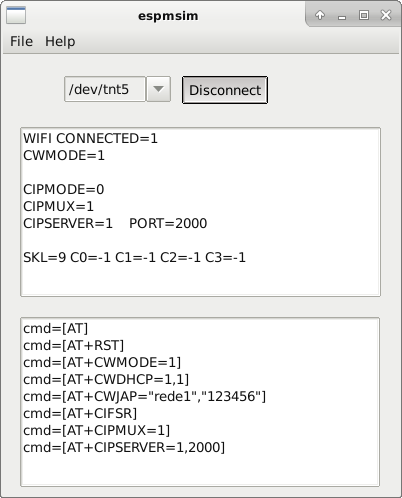
\includegraphics[width=0.7\textwidth]{img/espmsim.png} 
\end{figure} 

To use this tool with PICSimLab you first need to configure a virtual serial port as described in Chapter: \hyperlink{def:seriali}{Serial Communication}.
It is possible to use this tool with a real serial port connected to a real device. 


\subsection{Supported Commands}

\begin{itemize}
\item AT
\item AT+RST
\item AT+GMR
\item AT+CWMODE=1
\item AT+CWDHCP=1,1
\item AT+CWLAP
\item AT+CWJAP="rede1","123456"
\item AT+CIFSR
\item AT+CIPMUX=1
\item AT+CIPSERVER=1,2000
\item AT+CIPSEND=0,10
\item AT+CIPCLOSE=0
\end{itemize}


\section{Arduino Bootloader}\hypertarget{def:aboot}{}

This menu option load PICSimLab microcontroller with Arduino serial bootloader.  
The microcontroller with the bootloader loaded can be programmed directly by the 
Arduino IDE or using the avrdude program. 

To use this tool with PICSimLab you first need to configure a virtual serial port as described in Chapter: \hyperlink{def:seriali}{Serial Communication}.


\section{MPLABX Debugger Plugin} \hypertarget{def:mpdebug}{}

This menu option open the web page to download the MPLABX Debugger Plugin.

The plugin must be installed on MPLABX to allow debugging and programming 
PICSimLab (PICs and AVRs) from the IDE, like a real tool for debugging and 
programming.

\section{Pin Viewer} \hypertarget{def:pinv}{}

 The  PinViewer connects to PICSimLab through the \hyperlink{def:rcontrol}{rcontrol interface} 
 and allows viewing the status and direction of all microcontroller pins. 
 It is also possible to change the state of the digital pins and adjust the
 voltage value on the analog pins configured as input. Pins configured as outputs 
 also show the average value, useful for evaluating the functioning of PWM outputs. 
 
\begin{figure}[H]
\center
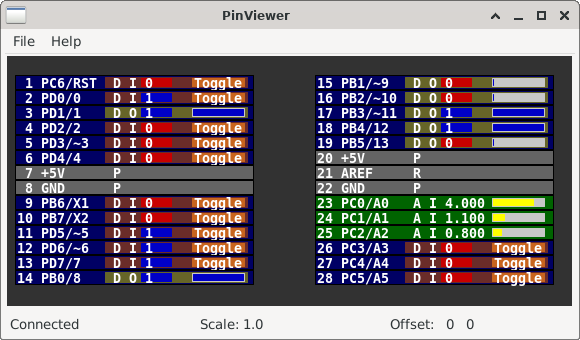
\includegraphics[width=0.7\textwidth]{img/pinviewer.png} 
\end{figure} 
